%Version 3.1 December 2024
% Migrated manuscript: Two Collapse Mechanisms for Non-Commutative Invariants of 3-SAT

\documentclass[pdflatex,sn-mathphys-num]{sn-jnl}

\usepackage{graphicx}%
\usepackage{amsmath,amssymb,amsfonts}%
\usepackage{booktabs}%
\usepackage{enumitem}%
\usepackage{tikz}%
\usetikzlibrary{positioning,arrows.meta,calc,backgrounds}%

\theoremstyle{thmstyleone}%
\newtheorem{theorem}{Theorem}%
\newtheorem{proposition}[theorem]{Proposition}%
\newtheorem{lemma}[theorem]{Lemma}%
\newtheorem{corollary}[theorem]{Corollary}%
\newtheorem{construction}[theorem]{Construction}%

\theoremstyle{thmstyletwo}%
\newtheorem{example}{Example}%
\newtheorem{remark}{Remark}%
\newtheorem{observation}[theorem]{Empirical Observation}%

\theoremstyle{thmstylethree}%
\newtheorem{definition}{Definition}%

\raggedbottom

% Running head (Springer / Algorithmica submission convention)
\makeatletter
\providecommand{\titlerunning}[1]{%
  \gdef\s@title{#1}%
  \markboth{\textit{#1}}{\textit{#1}}%
}
\makeatother

%-----------------------------------------------------------------------
%  Macros (preserved from original manuscript)
%-----------------------------------------------------------------------
\newcommand{\HH}{\mathbb{H}}
\newcommand{\QQ}{\mathbb{Q}}
\newcommand{\ZZ}{\mathbb{Z}}
\newcommand{\RR}{\mathbb{R}}
\newcommand{\NN}{\mathbb{N}}
\newcommand{\Nrd}{\operatorname{Nrd}}
\newcommand{\Trd}{\operatorname{Trd}}
\newcommand{\Tr}{\operatorname{Tr}}
\newcommand{\Sym}{\operatorname{Sym}}
\newcommand{\Ddet}{\operatorname{Ddet}}
\newcommand{\Fix}{\operatorname{Fix}}
\newcommand{\Det}{\operatorname{Det}}
\newcommand{\bi}{\mathbf{i}}
\newcommand{\bj}{\mathbf{j}}
\newcommand{\bk}{\mathbf{k}}
\newcommand{\Aphi}{A_{\varphi}}
\newcommand{\Gphi}{G_{\varphi}}
\newcommand{\Tphi}{T_{\varphi}}
\newcommand{\Vsat}{\mathcal{V}_{3\text{-}\mathrm{SAT}}}
% GitHub repository URL for the QIL workspace (edit before submission)
\newcommand{\QILRepositoryURL}{https://github.com/mauramyrez11/QIL-Research-Framework}
\DeclareMathOperator{\deggr}{deg}
\DeclareMathOperator{\spann}{span}
\DeclareMathOperator{\diag}{diag}
\DeclareMathOperator{\GL}{GL}
\DeclareMathOperator{\im}{Im}

\begin{document}

\title[Two Collapse Mechanisms for Non-Commutative Invariants of 3-SAT]{Two Collapse Mechanisms for Non-Commutative Invariants of 3-SAT: The Bipartite Gauge Involution and Terminal Abelianization in Quaternionic Incidence Matrices and Order-3 Tensors}
\titlerunning{Two Collapse Mechanisms for Non-Commutative Invariants of 3-SAT}

\author*[1]{\fnm{M.~M.} \sur{Paniagua-Ram\'irez}}\email{1912574a@umich.mx}

\affil*[1]{\orgdiv{Facultad de Ingenier\'ia El\'ectrica}, \orgname{Universidad Michoacana de San Nicol\'as de Hidalgo}, \orgaddress{\country{Mexico}}}

\abstract{We study why a natural class of non-commutative algebraic invariants fails
to separate satisfiable from unsatisfiable $3$-CNF formulas, using two
successive quaternionic encodings over the exact field $\QQ$. First, we
encode a formula's clause--variable incidence structure as a matrix over the
Hamiltonian quaternions $\HH(\QQ)$. We show that the bipartite two-colouring
of this structure induces a diagonal gauge involution that forces the
Dieudonn\'e determinant into a commutative subfield, annihilating all
inter-literal commutator torsion; we prove this collapse is intrinsic to any
bipartite bilinear encoding of width-$3$ clauses, and that avoiding it
forces the encoding's arity up to three. Second, we construct a symmetric
order-$3$ tensor encoding that removes this gauge symmetry and does retain
genuine non-commutative structure once vertex-degree heterogeneity breaks a
Fourier-theoretic cancellation on individual hyperedges. However, we show
that any scalar readout of this tensor factoring through the reduced
norm---including the Frobenius reduced-norm invariant and cyclic word-trace
invariants---projects the non-commutative spectrum onto a two-dimensional
commutative summary (reduced trace and reduced norm), discarding the oriented
information the construction was designed to preserve. We verify both
mechanisms on exact, size-matched satisfiable and unsatisfiable instances
using an open-source arbitrary-precision framework (QIL). The two
mechanisms---collapse in the object versus collapse in the
measurement---give a precise account of why this family of invariants cannot
separate $3$-SAT instances, and delineate constraints that any successor
invariant in this vein must satisfy.}

\keywords{non-commutative invariants, 3-SAT, quaternionic encodings, Dieudonn\'e determinant, geometric complexity theory, exact arithmetic}

\maketitle
%=======================================================================
\section{Introduction}\label{sec:intro}
%=======================================================================

\subsection{The \texorpdfstring{$\mathrm{P}$ versus $\mathrm{NP}$}{P vs NP} problem through
coordinate rings}

The Geometric Complexity Theory (GCT) program of Mulmuley and
Sohoni~\cite{GCT1,GCT2,MulmuleyCACM} reframes the $\mathrm{P}$ versus
$\mathrm{NP}$ separation, and complexity lower bounds more generally, as a
problem in the algebraic geometry of orbit closures. One attaches to a
computational object a point in a representation space, forms the closure
of its orbit under a natural group action, and seeks to separate two such
varieties---the orbit closure of a ``hard'' object and of an ``easy''
one---by exhibiting an \emph{explicit obstruction}: an element of the
coordinate ring, or a representation-theoretic multiplicity, that vanishes
identically on one variety but not the other. The strategic appeal of this
reformulation is that a genuine algebraic-geometric obstruction is designed
to slip past the three classical barriers that have blocked combinatorial
lower bounds: relativization~\cite{BGS}, the natural-proofs barrier of
Razborov and Rudich~\cite{RR}, and the algebrization barrier of Aaronson
and Wigderson~\cite{AW}.

The satisfiability problem $3$-SAT~\cite{Cook} is the canonical
$\mathrm{NP}$-complete anchor for such an attack: a $3$-CNF formula is a
finite, purely combinatorial object with an exact satisfiability label, so
any functional that decided satisfiability by thresholding a low-complexity
algebraic invariant would be an event of the first magnitude---and, by the
natural-proofs framework, an object one should expect not to exist in that
form. The value of the present work is precisely to make that expectation
\emph{structural and exact}: to build candidate invariants, run them
against exactly labelled instances with no numerical error whatsoever, and
then to prove, not merely observe, why they degenerate.

\subsection{Non-commutativity as structural rigidity}

In approaches motivated by GCT, a recurring obstacle is that linear
algebraic invariants over commutative fields are typically \emph{gauge
trivial}. Spectral data attached to an adjacency or incidence matrix $A$
are invariant under a similarity $A\mapsto U^{\dagger}AU$; the orbit of an
instance under such transformations collapses any spectral functional onto
a residue that cannot see the semantic distinctions between instances. This
illustrates, in miniature, a phenomenon structurally analogous to how
algebrization defeats algebraic-degree arguments~\cite{AW}: an invariant
computable from a
low-degree commutative extension inherits too much symmetry to separate
what it must.

Our program attacks this at the level of the coefficient ring. Rather than
diagonalising a matrix over a commutative cyclotomic field, we encode $3$-SAT
into structures over the \emph{rational Hamiltonian quaternion division
ring} $\HH(\QQ)$, mapping literal polarities onto anticommuting imaginary
units. Because $\bi\bj=-\bj\bi$, the linear reductions that trivialise
commutative spectra no longer act freely, and one may hope that a genuinely
non-commutative invariant---a Dieudonn\'e determinant~\cite{Dieudonne}, or a
non-abelian matrix word-trace---retains a rigid arithmetic datum that
distinguishes the satisfiability locus. The purpose of this paper is to
determine, with complete rigor and exact arithmetic, the fate of that hope.

\subsection{Two collapse mechanisms: a preview}

We report two distinct degeneration phenomena, discovered at two different
levels of the construction, and we argue that they are complementary poles
of a single taxonomy.

\begin{enumerate}
\item \textbf{Intrinsic Gauge Collapse} (matrix level,
Sections~\ref{sec:incidence}--\ref{sec:collapse}). The bipartite
clause--variable incidence matrix is a \emph{bilinear} object supported on
a two-colourable graph. That two-colouring \emph{is} a diagonal gauge
involution $\sigma_{\bk}(\Aphi)=G\Aphi G^{-1}$; it conjugates the
determinant representative into a commutative subfield and annihilates the
literal commutator torsion identically. The non-commutativity is destroyed
\emph{in the object itself}.

\item \textbf{Extrinsic Terminal Abelianization} (tensor level,
Sections~\ref{sec:tensor}--\ref{sec:terminal}). Passing to a symmetric
order-$3$ tensor removes the bipartite gauge---the object now genuinely
carries non-commutative structure, including surviving imaginary
components on unsatisfiable instances. Yet the \emph{scalar extraction}
used to read out a rational certificate---the reduced norm, or a reduced
norm of a word-trace---factors through the abelianization of
$\HH(\QQ)^{\times}$ and projects the non-commutative datum back onto the
commutative centre $\QQ$. The non-commutativity survives in the object but
is erased \emph{by the measurement}.
\end{enumerate}

Section~\ref{sec:bridge} is the logical hinge between the two: we prove that
the first collapse is not an accident of one matrix but an intrinsic
feature of order-$2$ formats, and that removing its cause forces the
transition to order-$3$ carriers, making the second phase inevitable rather
than optional.

\subsection{Reproducibility and exact arithmetic}

All exact computations, tensor constructions, quaternionic arithmetic,
invariant evaluations and reproducible experiments reported in this work
were performed using the \emph{Quaternionic Invariant Laboratory} (QIL), an
open-source exact-arithmetic research framework accompanying this
manuscript. Every numerical assertion below is the output of exact
computation over $\ZZ$ and $\QQ$ using arbitrary-precision integers and
fractions; there is no floating-point quantity at any stage, so all reduced
norms, traces, tensor entries, and invariants are exact rationals
reproducible bit-for-bit. The principal constructions are named in situ
(e.g.\ \texttt{build\_from\_cnf}, \texttt{compute\_dieudonne\_determinant},
\texttt{build\_tensor\_from\_cnf}, \texttt{contract\_axis},
\texttt{word\_trace}, \texttt{compute\_normalized\_invariant}). QIL is
described in Section~\ref{sec:software}, which also documents how every table
and figure in this paper can be regenerated.

\newpage

%=======================================================================
\section{The Quaternionic Incidence Model}\label{sec:incidence}
%=======================================================================

\subsection{The rational quaternion division ring}

Let $\HH(\QQ)=\QQ\oplus\QQ\bi\oplus\QQ\bj\oplus\QQ\bk$ be the Hamiltonian
quaternion algebra over the rationals~\cite{Voight}, with multiplication
fixed by Hamilton's relations
\begin{equation}\label{eq:hamilton}
  \bi^{2}=\bj^{2}=\bk^{2}=\bi\bj\bk=-1,\qquad
  \bi\bj=\bk=-\bj\bi,\quad \bj\bk=\bi=-\bk\bj,\quad \bk\bi=\bj=-\bi\bk.
\end{equation}
For $x=a+b\bi+c\bj+d\bk$ write the conjugate $\bar x=a-b\bi-c\bj-d\bk$ and
the reduced norm and reduced trace
\begin{equation}\label{eq:normtrace}
  \Nrd(x)=x\bar x=\bar x x=a^{2}+b^{2}+c^{2}+d^{2}\in\QQ_{\ge0},
  \qquad \Trd(x)=x+\bar x=2a.
\end{equation}
Since $\QQ$ is a formally real field, $\Nrd(x)=0\iff x=0$; every non-zero
$x$ is invertible with $x^{-1}=\Nrd(x)^{-1}\bar x$, so $\HH(\QQ)$ is a
division ring whose centre is exactly the scalar field $\QQ$. The reduced
norm is multiplicative, $\Nrd(xy)=\Nrd(x)\Nrd(y)$, a fact we shall use
repeatedly.

\begin{construction}[Quaternionic weights]\label{con:weights}
Weights are represented exactly as a canonical additive identity together
with a rational $4$-tuple $(a,b,c,d)$ otherwise. In the incidence model the
four components carry fixed structural semantics: $a$ is the scalar
(central) component, $b$ the positive-literal polarity on $\bi$, $c$ the
negative-literal polarity on $\bj$, and $d$ the clause structural index on
$\bk$. Arithmetic uses \eqref{eq:hamilton} and the exact inverse
$x^{-1}=\Nrd(x)^{-1}\bar x$.
\end{construction}

\subsection{The weighted bipartite incidence graph}

Let $\varphi=\bigwedge_{s=1}^{m}C_s$ be a $3$-CNF formula over Boolean
variables $x_0,\dots,x_{n-1}$, each clause
$C_s=\ell_{s,1}\vee\ell_{s,2}\vee\ell_{s,3}$ a disjunction of three
literals on distinct variables, each literal either positive ($x_v$) or
negative ($\lnot x_v$).

\begin{definition}[Weighted incidence graph]\label{def:graph}
The graph $\Gphi$ is the bipartite multigraph on
\[
  V=\underbrace{\{0,\dots,n-1\}}_{\text{variable vertices }V_0}
   \ \cup\
   \underbrace{\{n,\dots,n+m-1\}}_{\text{clause vertices }V_1},
\]
with $C_s$ identified with the vertex $n+s$. A variable vertex $v$ and a
clause vertex $n+s$ are adjacent iff some literal of $C_s$ is supported on
$x_v$, with weight $\bi$ if $x_v$ occurs positively and $\bj$ if
negatively. Each clause vertex carries the self-loop weight $\bk$.
\end{definition}

\begin{definition}[Algebraic adjacency matrix]\label{def:matrix}
The matrix $\Aphi\in\HH(\QQ)^{(n+m)\times(n+m)}$ is defined entrywise by
\[
  (\Aphi)_{p,q}=
  \begin{cases}
    \bi, & p<n\le q\ \text{and }x_p\in C_{q-n}\text{ positively (and symmetrically }(q,p)),\\
    \bj, & p<n\le q\ \text{and }x_p\in C_{q-n}\text{ negatively (and symmetrically }(q,p)),\\
    \bk, & p=q\ge n,\\
    \mathbf 0, & \text{otherwise.}
  \end{cases}
\]
Thus $\Aphi$ is symmetric; the variable--variable block and the whole
variable diagonal vanish; the clause--clause block is $\bk\,I_m$. It is
assembled by \texttt{build\_from\_cnf}.
\end{definition}

\begin{remark}\label{rem:cross}
Every cross (variable--clause) weight lies in
$\spann_\QQ\{\bi,\bj\}$, and every diagonal weight lies in
$\QQ\oplus\QQ\bk$. These two facts, together with the two-colouring
$(V_0,V_1)$, are the entire structural input to the collapse of
Section~\ref{sec:collapse}.
\end{remark}

%=======================================================================
\section{Global Torsion and the Commutative Collapse Theorem}
\label{sec:collapse}
%=======================================================================

Over a non-commutative division ring the ordinary determinant is
ill-defined; the correct substitute is the Dieudonn\'e
determinant~\cite{Dieudonne}, the universal multiplicative map
\[
  \Det:\GL_N(\HH(\QQ))\longrightarrow
       \HH(\QQ)^{\times}_{\mathrm{ab}}
       =\HH(\QQ)^{\times}\big/[\HH(\QQ)^{\times},\HH(\QQ)^{\times}],
\]
which for the Hamiltonian case is identified through the reduced norm with
$\QQ_{>0}$.

\subsection{A concrete representative by left-ordered elimination}

\begin{construction}[$\Ddet$ via left elimination]\label{con:ddet}
Set $M\gets\Aphi$ and $P\gets1$. For each pivot column $t=0,\dots,N-1$
($N=n+m$):
\begin{enumerate}[label=\textup{(\roman*)}]
\item \emph{Pivot search.} If $M_{t,t}=\mathbf0$, find the least $r>t$ with
$M_{r,t}\neq\mathbf0$, interchange rows $t,r$, and set $P\gets-P$; if none
exists, $\Aphi$ is singular and $\Ddet$ is undefined.
\item \emph{Left elimination.} For each $r>t$ with $M_{r,t}\neq\mathbf0$,
put $f\gets M_{r,t}M_{t,t}^{-1}$ and set
$M_{r,q}\gets M_{r,q}-fM_{t,q}$ for all $q\ge t$; since $fM_{t,t}=M_{r,t}$
this annihilates $M_{r,t}$.
\item \emph{Accumulation.} $P\gets P\cdot M_{t,t}$.
\end{enumerate}
Output $\Ddet(\Aphi)=P$.
\end{construction}

The order in (iii) matters: the pivots are accumulated as a left-to-right
ordered word in the non-commutative ring. The reduced norm
$\Nrd(\Ddet(\Aphi))=a^2+b^2+c^2+d^2\in\QQ_{>0}$ is independent of
elimination choices and is the canonical abelian Dieudonn\'e value; it is
computed by \texttt{dieudonne\_reduced\_norm}. All operations are exact in
$\QQ$.

\subsection{The conjugation involution and the bipartite gauge}

\begin{definition}\label{def:sigma}
Let $\sigma_{\bk}(x)=\bk x\bk^{-1}$ be conjugation by $\bk$.
\end{definition}

\begin{lemma}\label{lem:sigma}
$\sigma_{\bk}$ is a $\QQ$-algebra automorphism of $\HH(\QQ)$ with
\[
  \sigma_{\bk}(a+b\bi+c\bj+d\bk)=a-b\bi-c\bj+d\bk .
\]
Its fixed subring is the commutative field
$\Fix(\sigma_{\bk})=\QQ\oplus\QQ\bk\cong\QQ(\sqrt{-1})$, and its
$(-1)$-eigenspace is the literal plane $\spann_\QQ\{\bi,\bj\}$. Moreover
$\sigma_{\bk}(xy)=\sigma_{\bk}(x)\sigma_{\bk}(y)$ and
$\sigma_{\bk}(x^{-1})=\sigma_{\bk}(x)^{-1}$.
\end{lemma}

\begin{proof}
As an inner automorphism by a unit, $\sigma_{\bk}$ is a $\QQ$-algebra
automorphism, hence multiplicative and inversion-compatible. Using
$\bk^{-1}=-\bk$ and \eqref{eq:hamilton},
$\bk\bi\bk^{-1}=\bk\bi(-\bk)=-(\bk\bi)\bk=-\bj\bk=-\bi$, and similarly
$\bk\bj\bk^{-1}=-\bj$, while $\bk\bk\bk^{-1}=\bk$ and $\bk1\bk^{-1}=1$;
extend $\QQ$-linearly. An element is fixed iff $b=c=0$, i.e.\ lies in
$\QQ\oplus\QQ\bk$, and since $\bk^2=-1$ this subring is
$\QQ[x]/(x^2+1)\cong\QQ(\sqrt{-1})$; it is negated iff $a=d=0$.
\end{proof}

\begin{definition}[Bipartite gauge]\label{def:gauge}
Let $G=\diag(\varepsilon_0,\dots,\varepsilon_{N-1})\in\GL_N(\QQ)$ with
\[
  \varepsilon_p=\begin{cases}+1,&p<n\ (\text{variable vertex }V_0),\\
  -1,&p\ge n\ (\text{clause vertex }V_1).\end{cases}
\]
\end{definition}

\begin{lemma}[Gauge identity]\label{lem:gauge}
$\sigma_{\bk}(\Aphi)=G\,\Aphi\,G^{-1}$.
\end{lemma}

\begin{proof}
$G$ is central real diagonal, so
$(G\Aphi G^{-1})_{p,q}=\varepsilon_p\varepsilon_q^{-1}(\Aphi)_{p,q}
=\varepsilon_p\varepsilon_q(\Aphi)_{p,q}$ (as $\varepsilon_q=\pm1$). Compare
with $\sigma_{\bk}((\Aphi)_{p,q})$ by cases (Definition~\ref{def:matrix},
Lemma~\ref{lem:sigma}). For a variable--clause entry ($p<n\le q$ or
symmetric) the weight is $\bi$ or $\bj$, negated by $\sigma_{\bk}$, while
$\varepsilon_p\varepsilon_q=(+1)(-1)=-1$: both sides agree. For a clause
diagonal ($p=q\ge n$) the weight is $\bk$, fixed by $\sigma_{\bk}$, while
$\varepsilon_q\varepsilon_q=+1$: agreement. All remaining entries are
$\mathbf0$, fixed by both. Equality holds entrywise.
\end{proof}

\subsection{Propagation of the two-sided gauge through elimination}

\begin{lemma}[Two-sided gauge invariant]\label{lem:invariant}
At every step of Construction~\ref{con:ddet} the working matrix satisfies
$\sigma_{\bk}(M)=G_R\,M\,G_C^{-1}$, where $G_C=G$ is constant and
$G_R=\Pi G\Pi^{-1}$ for the cumulative row permutation $\Pi$. In particular
each pivot obeys $\sigma_{\bk}(M_{t,t})=\eta_t M_{t,t}$ with
$\eta_t=(G_R)_t(G_C)_t\in\{\pm1\}$, so $M_{t,t}\in\Fix(\sigma_{\bk})$ when
$\eta_t=+1$ and $M_{t,t}\in\spann_\QQ\{\bi,\bj\}$ when $\eta_t=-1$.
\end{lemma}

\begin{proof}
By Lemma~\ref{lem:gauge} the invariant holds initially with
$G_R=G_C=G$, $\Pi=\mathrm{id}$. We check each elementary operation.

\emph{Left elimination.} Write $\rho_p=(G_R)_p$, $\gamma_q=(G_C)_q$
($\pm1$), so $\sigma_{\bk}(M_{p,q})=\rho_p\gamma_q M_{p,q}$. The pivot obeys
$\sigma_{\bk}(M_{t,t})=\rho_t\gamma_t M_{t,t}$ and hence, by
Lemma~\ref{lem:sigma}, $\sigma_{\bk}(M_{t,t}^{-1})=\rho_t\gamma_t
M_{t,t}^{-1}$. For $f=M_{r,t}M_{t,t}^{-1}$,
\[
  \sigma_{\bk}(f)=\sigma_{\bk}(M_{r,t})\sigma_{\bk}(M_{t,t}^{-1})
  =(\rho_r\gamma_t M_{r,t})(\rho_t\gamma_t M_{t,t}^{-1})=\rho_r\rho_t f,
\]
using $\gamma_t^2=1$. Then for each $q\ge t$,
\[
  \sigma_{\bk}(fM_{t,q})=(\rho_r\rho_t f)(\rho_t\gamma_q M_{t,q})
  =\rho_r\gamma_q\, fM_{t,q},
\]
so $\sigma_{\bk}(M_{r,q}-fM_{t,q})=\rho_r\gamma_q(M_{r,q}-fM_{t,q})$; the
invariant is preserved with the same $G_R,G_C$.

\emph{Row interchange.} If $\Pi'$ swaps rows $t,r$ and $M'=\Pi'M$, then,
since $\Pi'$ is a real permutation matrix fixed by $\sigma_{\bk}$,
\[
  \sigma_{\bk}(M')=\Pi'\sigma_{\bk}(M)=\Pi'G_RMG_C^{-1}
  =(\Pi'G_R\Pi'^{-1})(\Pi'M)G_C^{-1}=(\Pi'G_R\Pi'^{-1})M'G_C^{-1},
\]
so $G_R\mapsto\Pi'G_R\Pi'^{-1}$ and $G_C$ is unchanged. Accumulation does
not alter $M$. Evaluating on the diagonal gives
$\sigma_{\bk}(M_{t,t})=\rho_t\gamma_t M_{t,t}=\eta_t M_{t,t}$, and
Lemma~\ref{lem:sigma} classifies the pivot.
\end{proof}

\subsection{The collapse}

\begin{theorem}[Commutative Collapse]\label{thm:collapse}
If $\Aphi$ is non-singular over $\HH(\QQ)$ then
$\Ddet(\Aphi)\in\QQ[\bk]=\QQ\oplus\QQ\bk\cong\QQ(\sqrt{-1})$; equivalently
its literal components vanish, $b=c=0$, whence
$\Nrd(\Ddet(\Aphi))=a^2+d^2$.
\end{theorem}

\begin{proof}
Write $\Ddet(\Aphi)=P=\varepsilon_\ast\prod_{t=0}^{N-1}p_t$, the ordered
product of pivots $p_t=M_{t,t}$ with global sign
$\varepsilon_\ast\in\{\pm1\}$ from row interchanges. By
Lemma~\ref{lem:invariant}, $\sigma_{\bk}(p_t)=\eta_t p_t$ with $\eta_t$
central, so, pulling the central scalars out of the ordered product,
\[
  \sigma_{\bk}(P)=\varepsilon_\ast\prod_t\sigma_{\bk}(p_t)
  =\varepsilon_\ast\Big(\prod_t\eta_t\Big)\prod_t p_t
  =\Big(\prod_t\eta_t\Big)P .
\]
It remains to evaluate the parity $\prod_t\eta_t$. Let $\Pi$ be the final
cumulative row permutation. The interchange used at column $t$ only swaps
rows of index $>t$, so once the pivot in position $t$ is read it is never
displaced; hence $(G_R)_t=\varepsilon_{\Pi(t)}$ and $(G_C)_t=\varepsilon_t$.
Therefore
\[
  \prod_{t}\eta_t=\prod_t\varepsilon_{\Pi(t)}\varepsilon_t
  =\Big(\prod_t\varepsilon_{\Pi(t)}\Big)\Big(\prod_t\varepsilon_t\Big)
  =\Big(\prod_s\varepsilon_s\Big)\Big(\prod_t\varepsilon_t\Big)
  =\Big(\prod_p\varepsilon_p\Big)^2=1,
\]
the third equality because $\Pi$ is a bijection (reindexing does not change
a product). Thus $\sigma_{\bk}(P)=P$, and by Lemma~\ref{lem:sigma}
$P\in\Fix(\sigma_{\bk})=\QQ[\bk]$, i.e.\ $b=c=0$; then
$\Nrd(a+d\bk)=a^2+d^2$.
\end{proof}

\begin{remark}\label{rem:parity}
The subtlety is that individual pivots need \emph{not} be central. The
identically-zero variable diagonal of $\Aphi$ forces interchanges with
clause rows of opposite gauge, producing literal-plane pivots
($\eta_t=-1$). The collapse holds not because each pivot is central but
because the number of such literal-plane pivots is \emph{even}, forced by
$\prod_t\eta_t=(\prod_p\varepsilon_p)^2=1$.
\end{remark}

\begin{example}[The parity mechanism at minimal size]\label{ex:elim}
To exhibit Construction~\ref{con:ddet} and the parity of
Remark~\ref{rem:parity} concretely, take the smallest incidence-type block
with a vanishing variable diagonal: one variable vertex ($V_0=\{0\}$) and
one clause vertex ($V_1=\{1\}$), joined by a positive-literal edge, so
\[
  A=\begin{pmatrix}\mathbf 0 & \bi\\[2pt] \bi & \bk\end{pmatrix},
  \qquad G=\diag(+1,-1).
\]
One checks $\sigma_{\bk}(A)=GAG^{-1}$ directly: the cross entries $\bi$
satisfy $\sigma_{\bk}(\bi)=-\bi$ and pick up $\varepsilon_0\varepsilon_1=-1$,
while the diagonal $\bk$ is $\sigma_{\bk}$-fixed and picks up
$\varepsilon_1\varepsilon_1=+1$. Running the elimination: at $t=0$ the pivot
$A_{0,0}=\mathbf 0$ forces a row swap ($P\gets-1$), yielding pivot
$p_0=\bi$ (a literal-plane pivot, $\eta_0=-1$) and the working matrix
$\bigl(\begin{smallmatrix}\bi&\bk\\ \mathbf0&\bi\end{smallmatrix}\bigr)$;
accumulation gives $P=(-1)\cdot\bi=-\bi$. At $t=1$ the pivot is
$p_1=\bi$ (again literal-plane, $\eta_1=-1$), and $P=(-\bi)\cdot\bi
=-\bi^2=1$. Thus $\Ddet(A)=1\in\QQ[\bk]$, with $b=c=0$ and torsion
$\tau=2bc=0$. The two literal-plane pivots occur in an \emph{even} number,
$\prod_t\eta_t=(-1)(-1)=+1$, exactly as Theorem~\ref{thm:collapse}
requires; their individual non-centrality is annihilated in the ordered
product.
\end{example}

\begin{example}[The torsion channel is live off the incidence locus]
\label{ex:live}
The vanishing of $\tau$ is a property of the incidence \emph{format}, not of
$\HH(\QQ)$. Consider the upper-triangular matrix
\[
  B=\begin{pmatrix}1+\bi & \bk\\[2pt] \mathbf 0 & 1+\bj\end{pmatrix},
\]
whose diagonal entries $1+\bi$ and $1+\bj$ lie \emph{outside}
$\Fix(\sigma_{\bk})$, violating hypothesis (iii) of
Definition~\ref{def:order2}. Being triangular, its Dieudonn\'e
representative is the ordered product of the diagonal,
\[
  \Ddet(B)=(1+\bi)(1+\bj)=1+\bj+\bi+\bi\bj=1+\bi+\bj+\bk,
\]
so $b=c=1$ and the commutator torsion is $\tau(B)=2bc=2\neq0$. Thus the
inter-literal torsion is a genuinely non-trivial functional on
$\HH(\QQ)$-matrices; it is precisely the two-colourable incidence geometry
(Theorem~\ref{thm:intrinsic}), not any deficiency of the ring, that forces
$\tau\equiv0$ in Corollary~\ref{cor:torsion}.
\end{example}

\subsection{Annihilation of the inter-literal commutator torsion}

The intended obstruction was the coupling of the two literal axes through
the non-commutative product.

\begin{definition}[Commutator torsion]\label{def:torsion}
For non-singular $\Aphi$ with $\Ddet(\Aphi)=a+b\bi+c\bj+d\bk$, the literal
projections $b\bi,c\bj$ have commutator
\[
  [\,b\bi,\,c\bj\,]=b\bi\,c\bj-c\bj\,b\bi=bc(\bi\bj-\bj\bi)=2bc\,\bk,
\]
so the torsion is $\tau(\Aphi)=2bc\in\QQ$; it is computed by
\texttt{compute\_annihilating\_functional}.
\end{definition}

\begin{corollary}[Identical annihilation]\label{cor:torsion}
For every non-singular incidence matrix, $\tau(\Aphi)=2bc\equiv0$, and the
radical $b^2+c^2+d^2$ reduces to $d^2$. The only surviving channel is the
soft scalar/clause magnitude $a^2+d^2$.
\end{corollary}

\begin{proof}
By Theorem~\ref{thm:collapse}, $b=c=0$; hence $2bc=0$ and
$b^2+c^2+d^2=d^2$.
\end{proof}

That the torsion channel is not \emph{a priori} trivial is confirmed by a
directly constructed non-incidence matrix with
$\Ddet=(1+\bi)(1+\bj)=1+\bi+\bj+\bk$, for which $b=c=1$ and $\tau=2\neq0$.
The incidence geometry, not the ring, is what annihilates it.

\subsection{The minimal control pair and non-persistence}

\begin{observation}[$3$-variable control pair]\label{obs:linpair}
Let $\varphi_{\mathrm{UNSAT}}$ be the conjunction of all eight sign patterns
on $\{x_0,x_1,x_2\}$ (the minimal unsatisfiable $3$-CNF) and
$\varphi_{\mathrm{SAT}}$ the same with the all-negative clause deleted.
Exact evaluation gives
\[
  \Nrd(\Ddet(A_{\varphi_{\mathrm{SAT}}}))=43264=2^{8}\cdot13^{2},
  \qquad
  \Nrd(\Ddet(A_{\varphi_{\mathrm{UNSAT}}}))=65536=2^{16}.
\]
The unsatisfiable norm is a pure power of two; the satisfiable one carries
the odd prime $13$.
\end{observation}

\begin{observation}[Non-persistence]\label{obs:linscale}
The pure-power phenomenon is not scale-invariant. At the random-$3$-SAT
critical ratio $\alpha=213/50\approx4.26$ (encoded exactly, with
$m=\lfloor213n/50\rfloor$), exact evaluation over sampled labelled
instances produces, for example, an unsatisfiable
$\Nrd=640000=2^{10}\cdot5^{4}$ whose odd prime $5$ violates any
``pure-power lemma'', while satisfiable norms exhibit their own odd primes.
Across a reproducible random corpus of $160$ critical-ratio instances ($20$
per variable count for $3\le n\le10$, checked by \texttt{stress\_tests}),
exact evaluation of $\Ddet(\Aphi)$ exhibits $b=c=0$ in every non-singular
case---in exact agreement with Theorem~\ref{thm:collapse}.
\end{observation}

Combining Theorem~\ref{thm:collapse} with
Observations~\ref{obs:linpair}--\ref{obs:linscale}, the entire
discriminatory content of the incidence construction is confined to the
imaginary-quadratic magnitude $a^2+d^2$, which varies with clause count and
carries no rigid arithmetic separation of the satisfiability locus.

\newpage

%=======================================================================
\section{The Inevitability of Trilinear Objects}\label{sec:bridge}
%=======================================================================

We now argue that Theorem~\ref{thm:collapse} is not a defect of one
encoding but an \emph{intrinsic} property of order-$2$ (matrix) formats of
the kind under consideration, and that removing its cause forces the arity
of the carrier up to three. This section is the logical bridge: it makes the
tensor phase a deduction rather than a fresh guess.

\subsection{The collapse generalises to all bipartite bilinear encodings}

\begin{definition}[Polarity-type order-$2$ encoding]\label{def:order2}
An \emph{order-$2$ incidence encoding} of $\varphi$ is a symmetric matrix
$A\in\HH(\QQ)^{V\times V}$ on a vertex set $V$ such that (i) the support
graph is bipartite with parts $(V_0,V_1)$, i.e.\ off-diagonal entries are
non-zero only between $V_0$ and $V_1$; (ii) every off-diagonal (cross)
entry lies in the literal plane $\spann_\QQ\{\bi,\bj\}=$ the
$(-1)$-eigenspace of $\sigma_{\bk}$; and (iii) every diagonal entry lies in
$\Fix(\sigma_{\bk})=\QQ\oplus\QQ\bk$.
\end{definition}

\begin{theorem}[Intrinsic bipartite gauge collapse]\label{thm:intrinsic}
For every non-singular order-$2$ incidence encoding $A$ (Definition
\ref{def:order2}) there is a diagonal involution $G=\diag(\varepsilon_p)$,
$\varepsilon_p=+1$ on $V_0$ and $-1$ on $V_1$, with
$\sigma_{\bk}(A)=GAG^{-1}$, and consequently $\Ddet(A)\in\QQ[\bk]$; in
particular the commutator torsion $\tau(A)=2bc$ vanishes identically.
\end{theorem}

\begin{proof}
As in Lemma~\ref{lem:gauge}, $G$ central gives
$(GAG^{-1})_{p,q}=\varepsilon_p\varepsilon_q A_{p,q}$. For a cross entry
($p\in V_0,q\in V_1$ or vice versa) condition (ii) makes $A_{p,q}$ lie in
the $(-1)$-eigenspace, $\sigma_{\bk}(A_{p,q})=-A_{p,q}$, while
$\varepsilon_p\varepsilon_q=-1$: agreement. For a diagonal entry condition
(iii) makes $\sigma_{\bk}(A_{p,q})=A_{p,q}$ while
$\varepsilon_p\varepsilon_q=+1$: agreement. Off-support entries are zero.
Hence $\sigma_{\bk}(A)=GAG^{-1}$, and the argument of
Lemmas~\ref{lem:invariant}, Theorem~\ref{thm:collapse} applies verbatim
(the elimination propagates the two-sided gauge and the parity product is a
square), forcing $\Ddet(A)\in\Fix(\sigma_{\bk})=\QQ[\bk]$ and $b=c=0$.
\end{proof}

Theorem~\ref{thm:intrinsic} says the collapse is a property of the
\emph{format}: any bilinear, bipartite, polarity-on-$\{\bi,\bj\}$ encoding
collapses, no matter how the clauses are wired. The incidence matrix of
Definition~\ref{def:matrix} is one instance; so is any reweighting that
respects (i)--(iii). Figure~\ref{fig:collapse} depicts the mechanism.

\begin{figure}[t]
\centering
\resizebox{\textwidth}{!}{%
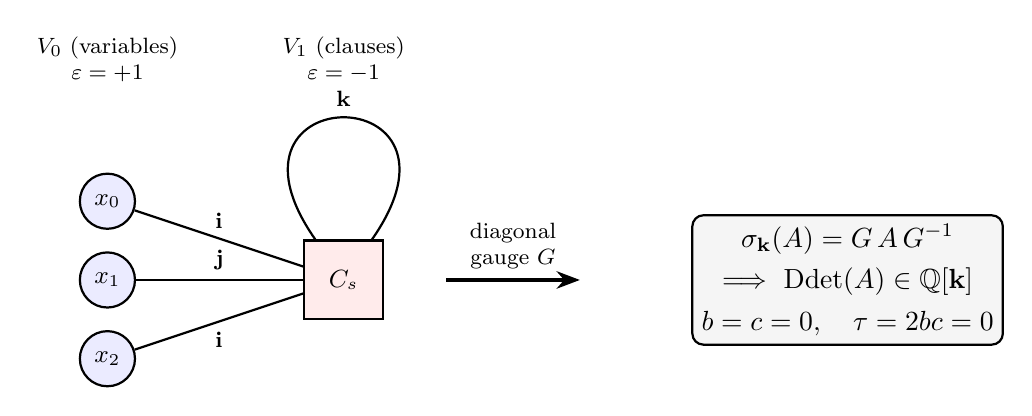
\begin{tikzpicture}[
  >=Stealth,
  var/.style={circle,draw,thick,minimum size=7mm,fill=blue!8,font=\small},
  cl/.style={rectangle,draw,thick,minimum size=10mm,fill=red!8,font=\small},
  lbl/.style={font=\footnotesize}
]
% variable vertices (gauge +1)
\node[var] (x0) at (0,2.0) {$x_0$};
\node[var] (x1) at (0,1.0) {$x_1$};
\node[var] (x2) at (0,0.0) {$x_2$};
\node[lbl,align=center] at (0,3.8) {$V_0$ (variables)\\ $\varepsilon=+1$};
% clause vertex (gauge -1)
\node[cl] (C) at (3,1.0) {$C_s$};
\node[lbl,align=center] at (3,3.8) {$V_1$ (clauses)\\ $\varepsilon=-1$};
% incidence edges, polarity on i / j
\draw[thick] (x0) -- node[lbl,above]{$\bi$} (C);
\draw[thick] (x1) -- node[lbl,above]{$\bj$} (C);
\draw[thick] (x2) -- node[lbl,below]{$\bi$} (C);
% structural self-loop k
\draw[thick] (C) to[out=55,in=125,looseness=9] node[lbl,above]{$\bk$} (C);
% gauge arrow
\draw[->,very thick] (4.3,1.0) -- node[lbl,align=center,above]{diagonal\\ gauge $G$} (6.0,1.0);
% collapsed state
\node[draw,thick,rounded corners,fill=gray!8,align=center] (box) at (9.4,1.0)
  {$\sigma_{\bk}(A)=G\,A\,G^{-1}$\\[3pt]
   $\Longrightarrow\ \Ddet(A)\in\QQ[\bk]$\\[3pt]
   $b=c=0,\quad \tau=2bc=0$};
\end{tikzpicture}%
}
\caption{The intrinsic bipartite gauge collapse
(Theorem~\ref{thm:intrinsic}). The two-colouring of the clause--variable
incidence graph into $V_0$ ($\varepsilon=+1$) and $V_1$ ($\varepsilon=-1$)
\emph{is} a diagonal involution $G=\diag(\varepsilon_p)$. Because the cross
weights $\bi,\bj$ lie in the $(-1)$-eigenspace of $\sigma_{\bk}$ and the
self-loop $\bk$ in its fixed field, conjugation by $G$ reproduces
$\sigma_{\bk}$ on $A$, forcing the Dieudonn\'e representative into the
commutative subfield $\QQ[\bk]$ and annihilating the literal commutator
torsion.}
\label{fig:collapse}
\end{figure}

\subsection{Why bilinearity forces bipartiteness for width-3 clauses}

The remaining question is whether one could keep an order-$2$ carrier but
break hypothesis (i), the bipartiteness. We argue that for a faithful
encoding of width-$3$ clauses this is impossible without reintroducing a
two-colouring.

\begin{proposition}[Arity obstruction]\label{prop:arity}
A symmetric order-$2$ array indexed by a single class of $n$ variable
vertices can record, in one entry, at most a \emph{pairwise} interaction of
two variables. To register the simultaneous, order-sensitive interaction of
the three literals of a clause $C_s$ in a single algebraic locus, an
order-$2$ encoding must introduce an auxiliary vertex $c_s$ adjacent to the
three variables of $C_s$; the resulting support graph is bipartite between
variables and auxiliary vertices, hence subject to
Theorem~\ref{thm:intrinsic}.
\end{proposition}

\begin{proof}
An entry $A_{p,q}$ of a matrix is a function of exactly the ordered pair
$(p,q)$ of indices; it cannot depend on a third index. Thus any single
matrix entry sees at most two variables. A width-$3$ clause is a $3$-ary
relation $R\subseteq\{0,\dots,n-1\}^3$ (its ordered support with polarities);
to attach one algebraic datum to the whole of $R$ within a matrix one must
route the three participating variables through a common index, i.e.\ a
vertex $c_s$ with edges $(c_s,i),(c_s,j),(c_s,k)$. The variable vertices
carry no mutual edges induced by $C_s$ (a matrix cannot place a single
weight on the unordered triple $\{i,j,k\}$), so the support of $C_s$ is a
star centred at $c_s$; the union over clauses is bipartite between
$\{c_s\}_s$ and the variables. Placing polarities on $\bi,\bj$ and the
clause marker on $\bk$ then satisfies (ii)--(iii), and
Theorem~\ref{thm:intrinsic} applies.
\end{proof}

\begin{corollary}[Necessity of order-$3$ carriers]\label{cor:necessity}
To encode the simultaneous three-literal interaction of a $3$-CNF clause
without an auxiliary vertex class---and hence without the bipartite gauge
of Theorem~\ref{thm:intrinsic}---the algebraic carrier must have internal
arity equal to the clause width. The minimal such carrier over a single
variable class is a symmetric order-$3$ tensor
$\Tphi\in(\HH(\QQ)^n)^{\otimes3}$, whose entry $(\Tphi)_{i,j,k}$ is indexed
by an ordered triple and can therefore hold one datum for the whole
hyperedge $\{i,j,k\}$.
\end{corollary}

Corollary~\ref{cor:necessity} is the deduction that drives the rest of the
paper: matching the internal dimension of the carrier to the clause width
eliminates the auxiliary clause class, hence the two-colouring, hence the
diagonal gauge involution. The price is that we leave the well-developed
theory of the Dieudonn\'e determinant and must construct new invariants for
a symmetric trilinear form---and, as we shall see, a \emph{second} and more
insidious collapse awaits at the moment of scalar extraction.

\newpage

%=======================================================================
\section{The Quaternionic Order-3 Tensor Construction}\label{sec:tensor}
%=======================================================================

\subsection{The 3-uniform hypergraph of a formula}

We reuse $\HH(\QQ)$ and its exact arithmetic. The vertices are now the
Boolean variables themselves, and each width-$3$ clause is a hyperedge on
three of them.

\begin{definition}[Variable degree]\label{def:degt}
$\deggr(v)$ is the number of literal occurrences of $v$ across $\varphi$,
independent of polarity.
\end{definition}

\begin{definition}[Order-3 tensor space]\label{def:tensorspace}
The state of the laboratory is a symmetric tensor
$\Tphi\in(\HH(\QQ)^{n})^{\otimes3}$ with entries
$(\Tphi)_{i,j,k}\in\HH(\QQ)$, $0\le i,j,k<n$, stored densely as $n^3$
exact quaternions. Symmetry means invariance under the $S_3$ action on the
three slots: $(\Tphi)_{i,j,k}=(\Tphi)_{\pi(i),\pi(j),\pi(k)}$ for all
$\pi\in S_3$.
\end{definition}

\subsection{Polarity embedding and non-local degree modulation}

The predecessor placed positive polarity on $\bi$ and negative on $\bj$.
We keep polarity on the imaginary axes but assign one axis per clause
\emph{position}, so the three literals occupy distinct anticommuting
directions, and we modulate by a non-local connectivity factor.

\begin{definition}[Clause weight]\label{def:weight}
For a clause $C_s$ with ordered variable support $(i,j,k)$ and signs
$(s_i,s_j,s_k)\in\{\pm1\}^3$, the connectivity factor and base weight are
\begin{equation}\label{eq:weight}
  D_s=\deggr(i)\deggr(j)\deggr(k)\in\ZZ_{>0},\qquad
  w_s=D_s\big(1+s_i\bi+s_j\bj+s_k\bk\big)\in\HH(\QQ).
\end{equation}
\end{definition}

The scalar $1$ is a sign-independent structural background; the signed units
$s_i\bi,s_j\bj,s_k\bk$ carry the three polarities on mutually anticommuting
axes; and $D_s$ couples the local hyperedge to the global vertex
connectivity, making $w_s$ a genuinely non-local functional of $\varphi$.
The rationale for the scalar background and the degree factor is developed
in Section~\ref{sec:fourier}; both are forced by the requirement that the
unsatisfiable control not annihilate.

\begin{definition}[Tensor assembly]\label{def:assembly}
With the $S_3$-symmetrization operator
$(\Sym U)_{i,j,k}=\tfrac16\sum_{\pi\in S_3}U_{\pi(i),\pi(j),\pi(k)}$ (an
exact rational average), the tensor of $\varphi$ is
\[
  \Tphi=\Sym\!\Big(\sum_{s=1}^{m}\sum_{\pi\in S_3}
     w_s\,E_{\pi(i_s,j_s,k_s)}\Big),
\]
where $E_{a,b,c}$ is the unit tensor at $(a,b,c)$ and $(i_s,j_s,k_s)$ the
ordered support of $C_s$. Equivalently each clause deposits $w_s$
additively onto all six permutations of its index triple; clauses sharing a
triple accumulate; the result is averaged over each $S_3$ orbit. This is
\texttt{build\_tensor\_from\_cnf}.
\end{definition}

Because each clause already deposits into all six permuted slots, the
pre-symmetrized tensor is $S_3$-invariant on non-degenerate triples and the
closing $\Sym$ is idempotent there; it also normalizes degenerate orbits
(with repeated indices) consistently. Figure~\ref{fig:lift} illustrates the
arity lift from a pairwise matrix incidence to a single trilinear tensor
slot.

\begin{figure}[t]
\centering
\resizebox{\textwidth}{!}{%
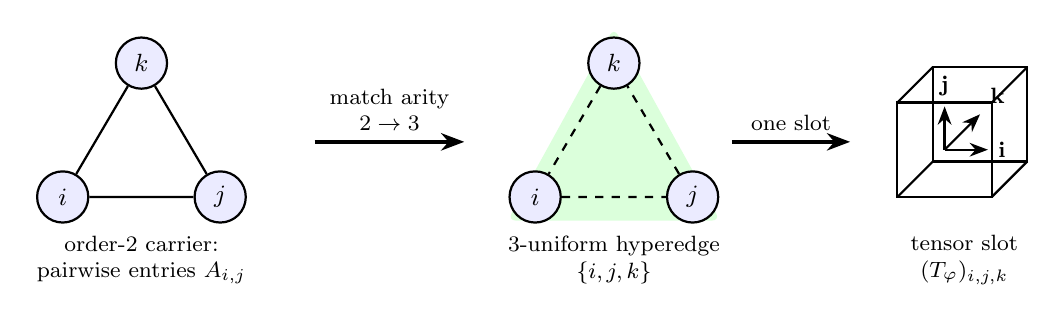
\begin{tikzpicture}[
  >=Stealth,
  v/.style={circle,draw,thick,fill=blue!8,minimum size=6.5mm,font=\small},
  lbl/.style={font=\footnotesize}
]
% --- left: order-2 pairwise edges ---
\node[v] (a) at (0,0)   {$i$};
\node[v] (b) at (2,0)   {$j$};
\node[v] (c) at (1,1.7) {$k$};
\draw[thick] (a)--(b) (b)--(c) (c)--(a);
\node[lbl,align=center] at (1,-0.8) {order-2 carrier:\\ pairwise entries $A_{i,j}$};

% --- arrow ---
\draw[->,very thick] (3.2,0.7) -- node[lbl,align=center,above]{match arity\\ $2\to3$} (5.1,0.7);

% --- middle: 3-uniform hyperedge ---
\begin{scope}[xshift=6cm]
  \node[v] (a2) at (0,0)   {$i$};
  \node[v] (b2) at (2,0)   {$j$};
  \node[v] (c2) at (1,1.7) {$k$};
  \begin{scope}[on background layer]
    \fill[green!14,rounded corners=3pt]
      ($(a2)+(-0.35,-0.30)$) -- ($(b2)+(0.35,-0.30)$) -- ($(c2)+(0,0.45)$) -- cycle;
  \end{scope}
  \draw[thick,dashed] (a2)--(b2) (b2)--(c2) (c2)--(a2);
  \node[lbl,align=center] at (1,-0.8) {3-uniform hyperedge\\ $\{i,j,k\}$};
\end{scope}

% --- arrow to tensor slot ---
\draw[->,very thick] (8.5,0.7) -- node[lbl,align=center,above]{one slot} (10.0,0.7);

% --- right: order-3 tensor slot (isometric cube) ---
\begin{scope}[xshift=10.6cm,yshift=0.0cm]
  \def\d{0.45}
  \draw[thick] (0,0) rectangle (1.2,1.2);
  \draw[thick] (\d,\d) rectangle (1.2+\d,1.2+\d);
  \draw[thick] (0,0)--(\d,\d) (1.2,0)--(1.2+\d,\d)
               (1.2,1.2)--(1.2+\d,1.2+\d) (0,1.2)--(\d,1.2+\d);
  % axes inside
  \draw[->,thick] (0.6,0.6)--(1.15,0.6) node[right,lbl]{$\bi$};
  \draw[->,thick] (0.6,0.6)--(0.6,1.15) node[above,lbl]{$\bj$};
  \draw[->,thick] (0.6,0.6)--(0.6+\d,0.6+\d) node[above right,lbl]{$\bk$};
  \node[lbl,align=center] at (0.85,-0.8) {tensor slot\\ $(\Tphi)_{i,j,k}$};
\end{scope}
\end{tikzpicture}%
}
\caption{From a bilinear adjacency graph to a trilinear tensor slot. A
matrix entry $A_{i,j}$ can bind only a \emph{pair} of vertices (left), so a
width-$3$ clause must be split across pairwise incidences; lifting the
carrier's arity to match the clause width represents the clause as a single
$3$-uniform hyperedge $\{i,j,k\}$ (centre), stored in one symmetric order-3
tensor slot $(\Tphi)_{i,j,k}$ whose three axes carry the anticommuting
generators $\bi,\bj,\bk$ (right).}
\label{fig:lift}
\end{figure}

\begin{proposition}[Disappearance of the bipartite gauge]\label{prop:nogauge}
There is no single-class analogue of the diagonal gauge of
Theorem~\ref{thm:intrinsic} for $\Tphi$. Concretely, the involution
$\sigma_{\bk}$ acts on each entry by $a+b\bi+c\bj+d\bk\mapsto a-b\bi-c\bj+d\bk$,
and for a clause with mixed polarity the entry $w_s/D_s=1+s_i\bi+s_j\bj+s_k\bk$
is neither fixed nor negated by $\sigma_{\bk}$; hence no central diagonal
$G$ can satisfy $\sigma_{\bk}(\Tphi)_{i,j,k}=\varepsilon_i\varepsilon_j
\varepsilon_k(\Tphi)_{i,j,k}$ uniformly across the orbit.
\end{proposition}

\begin{proof}
Take a clause with $(s_i,s_j,s_k)=(+1,-1,+1)$, so the entry is proportional
to $1+\bi-\bj+\bk$, with $\sigma_{\bk}$-image $1-\bi+\bj+\bk$. If a central
scalar $\varepsilon\in\{\pm1\}$ satisfied
$\sigma_{\bk}(1+\bi-\bj+\bk)=\varepsilon(1+\bi-\bj+\bk)$, comparing scalar
parts gives $\varepsilon=+1$, but then the $\bi$-parts give $-1=+1$, a
contradiction. Thus no single-class diagonal conjugation reproduces
$\sigma_{\bk}$ on $\Tphi$, and the mechanism of Theorem~\ref{thm:intrinsic}
does not transport.
\end{proof}

Proposition~\ref{prop:nogauge} confirms that the transition of
Section~\ref{sec:bridge} achieved its structural aim: the intrinsic gauge
collapse is gone. We now show that a subtler obstacle takes its place.

\newpage

%=======================================================================
\section{Fourier Hypercube Annihilation and Degree Heterogeneity}
\label{sec:fourier}
%=======================================================================

\subsection{The annihilation on a symmetric hyperedge}

Fix a variable triple $\{i,j,k\}$. By Definition~\ref{def:assembly} the
orbit entry $(\Tphi)_{i,j,k}$ is the sum of the base weights of all clauses
supported on that triple; when all such clauses share the triple, their
$D_s$ share the common value $D=\deggr(i)\deggr(j)\deggr(k)$. If the set of
sign patterns is $\Sigma\subseteq\{\pm1\}^3$ then
\begin{equation}\label{eq:orbitsum}
  (\Tphi)_{i,j,k}
   =D\sum_{\sigma\in\Sigma}\big(1+\sigma_1\bi+\sigma_2\bj+\sigma_3\bk\big)
   =D\Big(|\Sigma|+\big(\textstyle\sum_\sigma\sigma_1\big)\bi
      +\big(\sum_\sigma\sigma_2\big)\bj+\big(\sum_\sigma\sigma_3\big)\bk\Big).
\end{equation}

\begin{theorem}[Fourier Hypercube Annihilation]\label{thm:annih}
If the clauses on a triple enumerate the full sign cube
$\Sigma=\{\pm1\}^3$ with uniform multiplicity, the orbit entry is a pure
real scalar,
\[
  (\Tphi)_{i,j,k}=D\cdot2^{3}=8D\in\QQ\subset\HH(\QQ),
\]
and all imaginary (non-central) components vanish identically.
\end{theorem}

\begin{proof}
Each coordinate map $\sigma\mapsto\sigma_r$ is a non-trivial character of
the abelian group $(\{\pm1\}^3,\cdot)$, so by orthogonality of
characters~\cite{ODonnell}, $\sum_{\sigma\in\{\pm1\}^3}\sigma_r=0$ for
$r=1,2,3$. Substituting $|\Sigma|=8$ into \eqref{eq:orbitsum} annihilates
the $\bi,\bj,\bk$ terms and leaves $8D$ on the scalar axis.
\end{proof}

Equivalently, over the full cube every first-order (odd) Fourier mode of
$\sigma\mapsto1+\sum_r\sigma_r\mathbf e_r$ integrates to zero, leaving only
the constant mode. This is exactly why the base weight \eqref{eq:weight}
includes the scalar unit $1$: without it the entry would vanish outright on
the symmetric control, and \emph{with} it the entry retains a non-zero
(albeit purely real) value equal to $D$ times the clause count.

\begin{observation}[Minimal control pair, $n=3$]\label{obs:n3}
Let $\varphi_{\mathrm{UNSAT}}$ be all eight sign patterns on
$\{x_0,x_1,x_2\}$ and $\varphi_{\mathrm{SAT}}$ the same minus the
all-negative clause. Here every clause spans the same triple, so degrees are
uniform: $\deggr\equiv8$ (UNSAT, $m=8$, $D=512$) and $\deggr\equiv7$ (SAT,
$m=7$, $D=343$). On each of the six non-degenerate orbit entries,
\[
  (\Tphi^{\mathrm{UNSAT}})_{i,j,k}=512\cdot8=4096\in\QQ,\qquad
  (\Tphi^{\mathrm{SAT}})_{i,j,k}=343(7+\bi+\bj+\bk)=2401+343\bi+343\bj+343\bk.
\]
The unsatisfiable tensor is a pure real scalar, exactly as
Theorem~\ref{thm:annih} predicts; the satisfiable one retains a residual
multi-vector only because one clause is \emph{missing}, breaking the
full-cube balance. The exact squared Frobenius separation is
$\sum_{i,j,k}\Nrd\big((\Tphi^{\mathrm{SAT}}-\Tphi^{\mathrm{UNSAT}})_{i,j,k}\big)
=6\,(1695^2+3\cdot343^2)=19{,}355{,}832$.
\end{observation}

\subsection{Degree heterogeneity shatters the local cancellation}

Theorem~\ref{thm:annih} concerns a single hyperedge that sees the balanced
cube. For $n\ge4$ the formula spreads across several triples, which forces
heterogeneous degrees and ensures that auxiliary triples are covered only
by a proper (unbalanced) subset of sign patterns.

\begin{proposition}[Survival of quaternionic structure]\label{prop:survive}
Suppose a triple $\{i,j,k\}$ carries a sign set
$\Sigma\subsetneq\{\pm1\}^3$ with $\sum_{\sigma\in\Sigma}\sigma_r\neq0$ for
some $r$. Then $(\Tphi)_{i,j,k}$ has a non-zero component of magnitude
$D\,|\sum_\sigma\sigma_r|$ on axis $r$, with
$D=\deggr(i)\deggr(j)\deggr(k)$. Heterogeneous degrees rescale distinct
triples by distinct factors $D$, so no single central rescaling can
simultaneously annihilate them.
\end{proposition}

\begin{proof}
Immediate from \eqref{eq:orbitsum}: the axis-$r$ component equals
$D\sum_{\sigma\in\Sigma}\sigma_r\neq0$. Distinct triples of differing
degree carry distinct $D$, so the imaginary pattern is not a common scalar
multiple of a single cancelling profile.
\end{proof}

\begin{observation}[Heterogeneous pair, $n=4$]\label{obs:n4}
Let $\varphi_{\mathrm{UNSAT}}$ consist of the eight patterns on
$\{0,1,2\}$ (which alone force unsatisfiability) together with
$(x_0\vee x_2\vee x_3)$, $(x_0\vee x_2\vee\lnot x_3)$,
$(\lnot x_1\vee x_2\vee x_3)$. The degree profile is
$(\deggr0,\deggr1,\deggr2,\deggr3)=(10,9,11,3)$, manifestly non-uniform.
Exact evaluation yields a pure real scalar on the balanced core triple and
genuine multi-vectors on the auxiliary triples:
\[
  (\Tphi)_{0,1,2}=990\cdot8=7920,\quad
  (\Tphi)_{0,2,3}=660+660\bi+660\bj,\quad
  (\Tphi)_{1,2,3}=297-297\bi+297\bj+297\bk,
\]
with $D_{012}=10\cdot9\cdot11=990$, $D_{023}=10\cdot11\cdot3=330$ (two
clauses, axis sums $(2,2,0)$), $D_{123}=9\cdot11\cdot3=297$ (one clause,
signs $(-,+,+)$). Twelve of the $64$ entries carry non-zero imaginary
parts: the annihilation barrier is shattered on the unsatisfiable side.
\end{observation}

\begin{remark}\label{rem:honest}
The honest content of Proposition~\ref{prop:survive} is that survival is
driven by \emph{local sign imbalance} (partial cube coverage), while degree
heterogeneity supplies the distinct scale factors $D$ that prevent a single
central gauge from re-annihilating the ensemble. The two effects are
logically distinct; heterogeneity is what makes partial coverage generic
for $n\ge4$. This nuance matters for Section~\ref{sec:discussion}: the
surviving structure is genuine but is driven by connectivity, not by
satisfiability.
\end{remark}


\newpage

%=======================================================================
\section{Non-Commutative Contraction and the Spectrum}\label{sec:contract}
%=======================================================================

To obtain a basis-independent scalar rather than comparing $n^3$ entries we
contract $\Tphi$ to a matrix and take a trace-type invariant.

\begin{definition}[Transverse contraction]\label{def:contract}
Given $V=(V_0,\dots,V_{n-1})\in\HH(\QQ)^n$, the induced marginal matrix
$M=M(V)\in\HH(\QQ)^{n\times n}$ is
\begin{equation}\label{eq:contract}
  M_{i,j}=\sum_{k=0}^{n-1}(\Tphi)_{i,j,k}\cdot V_k,
\end{equation}
each product taken in the fixed Hamiltonian order (tensor entry left, test
component right). The \emph{canonical spatial vector} is $V=[\bi,\bj,\bk,1]$
for $n=4$, extended cyclically ($V_k\in\{\bi,\bj,\bk,1\}$ by $k\bmod4$) for
general $n$. This is \texttt{contract\_axis}.
\end{definition}

Contracting against the imaginary generators probes the anticommuting axes
asymmetrically, so $M$ genuinely inhabits the non-commutative ring.

\begin{definition}[Two scalar extractions]\label{def:invariants}
For the marginal $M=M(V)$ we consider:
\begin{enumerate}
\item the \emph{Frobenius reduced-norm}
$\Phi(\Tphi)=\sum_{i,j}\Nrd(M_{i,j})\in\QQ_{\ge0}$, a cell-by-cell aggregate
(\texttt{reduced\_norm\_sum});
\item the \emph{non-commutative word-trace}: form the ordered power
$M^p$ by $(M^2)_{i,j}=\sum_k M_{i,k}M_{k,j}$, take the cyclic trace
$\Tr(M^p)=\sum_i(M^p)_{i,i}\in\HH(\QQ)$, and reduce to
$\Psi_p(\Tphi)=\Nrd\big(\Tr(M^p)\big)\in\QQ_{\ge0}$ (\texttt{word\_trace}
with $p=3$).
\end{enumerate}
For size normalization against $m$ clauses we use
$\widehat\Phi=\Phi/m^2$ and $\widehat\Psi_p=\Psi_p/m^2$, exact in $\QQ$
(\texttt{compute\_normalized\_invariant}).
\end{definition}

The reduced norm is the abelianization map
$\HH(\QQ)^{\times}\to\QQ_{>0}$: it factors through the commutator quotient
and satisfies $\Nrd(xy)=\Nrd(x)\Nrd(y)=\Nrd(yx)$, so $\Phi$ discards the
non-commutative content by construction. The word-trace $\Psi_p$ retains
non-abelian information \emph{inside} $M^p$ (assembled from ordered products
that do not commute), but the terminal $\Nrd$ re-abelianizes the endpoint.
Section~\ref{sec:terminal} shows this terminal projection is fatal;
Section~\ref{sec:experiments} shows it empirically.

\newpage

%=======================================================================
\section{The Terminal Abelianization Theorem}\label{sec:terminal}
%=======================================================================

We now elevate the empirical failure into a structural theorem: any scalar
extraction that factors through the reduced norm collapses the entire
non-commutative spectrum of the contracted matrix onto a
conjugation-invariant central pair, and is therefore blind to the oriented
data the quaternionic encoding preserves.

\subsection{Conjugacy invariance of the reduced norm}

\begin{lemma}[Conjugation invariance]\label{lem:conjinv}
For all $x\in\HH(\QQ)$ and units $u\in\HH(\QQ)^{\times}$,
\[
  \Trd(uxu^{-1})=\Trd(x),\qquad \Nrd(uxu^{-1})=\Nrd(x).
\]
\end{lemma}

\begin{proof}
Multiplicativity of $\Nrd$ gives
$\Nrd(uxu^{-1})=\Nrd(u)\Nrd(x)\Nrd(u)^{-1}=\Nrd(x)$, since $\Nrd$ takes
values in the commutative group $\QQ_{>0}$. For the trace, conjugation is a
$\QQ$-algebra automorphism (inner), hence commutes with the anti-involution
$x\mapsto\bar x$ and fixes the centre, so
$\Trd(uxu^{-1})=uxu^{-1}+\overline{uxu^{-1}}
=u(x+\bar x)u^{-1}=u\,\Trd(x)\,u^{-1}=\Trd(x)$ as $\Trd(x)\in\QQ$ is
central.
\end{proof}

\begin{lemma}[Conjugacy classes are level sets of $(\Trd,\Nrd)$]
\label{lem:levelsets}
Two elements $x,y\in\HH(\QQ)$ with $\im(x),\im(y)\neq0$ are conjugate over
$\HH(\RR)$ if and only if $\Trd(x)=\Trd(y)$ and $\Nrd(x)=\Nrd(y)$. Writing
$x=a+\vec v$ with $\vec v=b\bi+c\bj+d\bk$ the imaginary part, the map
\[
  x\longmapsto\big(\Trd(x),\Nrd(x)\big)=\big(2a,\ a^2+\lVert\vec v\rVert^2\big)
\]
is constant on the conjugation orbit of $x$, and the orbit of a
non-central $x$ is the $2$-sphere $\{a\}\times\{\vec w:\lVert\vec
w\rVert=\lVert\vec v\rVert\}$ of imaginary vectors of fixed length.
\end{lemma}

\begin{proof}
Conjugation by a unit acts trivially on the scalar part $a$ (the centre)
and as a rotation in $SO(3)$ on the imaginary part $\vec v$: for a unit
quaternion $u$, the map $\vec v\mapsto u\vec vu^{-1}$ is the standard
double cover $\HH^{\times}\to SO(3)$ acting on $\im\HH\cong\RR^3$, which
preserves $\lVert\vec v\rVert$ and realises every rotation. Hence the orbit
of $a+\vec v$ is exactly $\{a+\vec w:\lVert\vec w\rVert=\lVert\vec
v\rVert\}$, a $2$-sphere, on which $\Trd=2a$ and
$\Nrd=a^2+\lVert\vec v\rVert^2$ are constant; conversely equal
$(\Trd,\Nrd)$ forces equal $a$ and equal $\lVert\vec v\rVert$, hence
conjugacy.
\end{proof}

\subsection{The terminal collapse}

\begin{theorem}[Terminal Abelianization]\label{thm:terminal}
Let $\Tphi$ be any tensor and let $M=M(V)$ be a marginal obtained by the
linear contraction \eqref{eq:contract}. Let $t_p=\Tr(M^p)\in\HH(\QQ)$ be its
cyclic word-trace and let $F:\HH(\QQ)\to\QQ$ be any function that factors
through the reduced norm, i.e.\ $F=g\circ\Nrd$ for some $g:\QQ\to\QQ$ (in
particular $F=\Nrd$, or $F=\Nrd$ post-composed with normalization by
$m^2$). Then $F(t_p)$ depends on $t_p$ only through the
conjugation-invariant central pair $(\Trd(t_p),\Nrd(t_p))\in\QQ^2$; that is,
$F$ is constant on the entire $\HH(\QQ)^{\times}$-conjugation orbit of
$t_p$, and in particular is invariant under every $SO(3)$ rotation of the
imaginary part $\im(t_p)$. Consequently the scalar certificate retains, at
most, the two commutative numbers $(\Trd(t_p),\Nrd(t_p))$ and discards all
oriented (non-commutative) information carried by $\im(t_p)$.
\end{theorem}

\begin{proof}
By Lemma~\ref{lem:conjinv}, $\Nrd$ is constant on the conjugation orbit of
$t_p$; hence so is $F=g\circ\Nrd$. By Lemma~\ref{lem:levelsets} that orbit
is the full $2$-sphere of imaginary vectors of length
$\lVert\im(t_p)\rVert$ at fixed scalar part, on which $\Nrd$ takes the
single value $a^2+\lVert\im(t_p)\rVert^2$ and $\Trd$ the value $2a$. Thus
$F(t_p)$ is a function of $(a,\lVert\im(t_p)\rVert^2)$ alone, equivalently
of $(\Trd(t_p),\Nrd(t_p))$. Any two traces related by an inner
automorphism---equivalently, differing by a rotation of the imaginary
triple $(b,c,d)$---yield the same certificate. The three imaginary
components enter only through the isotropic combination
$b^2+c^2+d^2=\lVert\im(t_p)\rVert^2$, so the oriented content (the relative
phase among $\bi,\bj,\bk$ that encodes non-commutative order) is erased.
\end{proof}

\begin{example}[Orientation erasure]\label{ex:erase}
The three quaternions
\[
  t=3+4\bi,\qquad t'=3+4\bj,\qquad t''=3+4\bk
\]
are pairwise distinct and point along three mutually orthogonal imaginary
directions, encoding entirely different non-commutative phases. Yet
\[
  \Trd(t)=\Trd(t')=\Trd(t'')=6,\qquad
  \Nrd(t)=\Nrd(t')=\Nrd(t'')=3^2+4^2=25,
\]
so any certificate $F=g\circ\Nrd$ assigns them the identical value
$g(25)$. Were $\Tr(M^3)$ to equal $t$ for a satisfiable instance and $t'$
for an unsatisfiable one, the terminal reduced norm could not tell them
apart. More generally, the level set $\{a+\vec w:\lVert\vec
w\rVert^2=16\}$ at $a=3$ is an entire $2$-sphere of traces collapsed to the
single value $25$; the readout sees only the radius, never the direction.
\end{example}

\begin{corollary}[Extrinsic collapse]\label{cor:extrinsic}
Even when $M$ and $M^p$ carry non-trivial non-commutative structure---so
that $t_p\notin\QQ$---the certificate $\widehat\Psi_p=\Nrd(t_p)/m^2$ is a
function of the two central rationals $(\Trd(t_p),\Nrd(t_p))$ only. The
non-commutativity is destroyed not in the object but in the measurement;
we call this an \emph{extrinsic} collapse, in contradistinction to the
intrinsic gauge collapse of Theorem~\ref{thm:collapse}.
\end{corollary}

\begin{proof}
Immediate from Theorem~\ref{thm:terminal} with $F=\Nrd$ followed by division
by the central constant $m^2$.
\end{proof}

\subsection{Connection to the algebrization barrier}

Theorem~\ref{thm:terminal} illustrates, in miniature and with complete rigor,
a phenomenon structurally analogous to the algebrization barrier~\cite{AW}.
The construction was
engineered to be non-commutative so as to resist linear gauge symmetry; the
tensor phase even succeeds in keeping the object non-commutative
(Proposition~\ref{prop:nogauge}, Observation~\ref{obs:n4}). But the only
$\QQ$-valued, basis-independent readout available through the reduced norm
projects onto the centre, and the centre is a commutative field of low
degree ($\Nrd$ is a quadratic form). A separating obstruction, if it lives
downstream of such a readout, is therefore computable from a low-degree
commutative extension---precisely the regime against which algebrization is
provably effective, and, via Razborov--Rudich~\cite{RR}, the regime in which
a smoothly varying separating functional would constitute a natural
property. The failure mode is not that the object is too simple; it is that the
\emph{measurement} is abelian.

\newpage

%=======================================================================
\section{Exact Size-Matched Experiments}\label{sec:experiments}
%=======================================================================

\subsection{Methodology}

The Quaternionic Invariant Laboratory (QIL, Section~\ref{sec:software})
performs every computation over $\ZZ$ and $\QQ$ with arbitrary-precision
integers and fractions; no floating-point primitive appears anywhere, so all
reported quantities are exact and reproducible. Random $3$-CNF instances are
produced by a deterministic SplitMix64 integer stream (\texttt{random\_3cnf})
and labelled by an exhaustive exact solver (\texttt{is\_satisfiable}) scanning
all $2^n$ assignments. The two tables below are regenerated exactly by the
commands \texttt{cargo run -{}-example reproduce\_table\_1} and
\texttt{reproduce\_table\_2}. To isolate logical contradiction from brute
volumetric size, the harness holds the instance size perfectly constant:
every sample has $n=4$ variables and exactly $m=10$ clauses, drawn until a
fixed number of verified satisfiable and unsatisfiable instances is
collected. Because $m$ is constant across the batch, the normalization by
$m^2$ is a common constant within the batch and cannot by itself alter class
separation; it is retained so that batches of different size remain
comparable.

\subsection{Data}

Table~\ref{tab:frob} reports the abelian Frobenius invariant
$\widehat\Phi=\Phi/m^2$ and Table~\ref{tab:trace} the non-commutative
word-trace invariant $\widehat\Psi_3=\Nrd(\Tr(M^3))/m^2$, both as exact
rationals, sorted ascending within each satisfiability class, on the same
size-matched batch. The right-hand column gives the decimal magnitude as a
reading aid only; the exact rationals are the authoritative values.

\begin{table}[t]
\caption{Abelian Frobenius reduced-norm invariant $\widehat{\Phi}$,
size-matched ($n=4$, $m=10$), sorted ascending within each class. The
satisfiable band $[5.35,\,10.82]\times10^{5}$ and the unsatisfiable band
$[3.36,\,7.89]\times10^{5}$ share the common interval
$[5.35,\,7.89]\times10^{5}$, which contains members of both classes.}
\label{tab:frob}
\centering
\small
\begin{tabular}{@{}l l r@{}}
\toprule
Status & $\widehat{\Phi}=\Phi/m^{2}$ (exact rational) & Approx.\\
\midrule
SAT   & $13369344/25$   & $5.35\times10^{5}$\\
SAT   & $3493504/5$     & $6.99\times10^{5}$\\
SAT   & $780864$        & $7.81\times10^{5}$\\
SAT   & $20499738/25$   & $8.20\times10^{5}$\\
SAT   & $20715828/25$   & $8.29\times10^{5}$\\
SAT   & $27062016/25$   & $1.08\times10^{6}$\\
\midrule
UNSAT & $8410752/25$    & $3.36\times10^{5}$\\
UNSAT & $13284096/25$   & $5.31\times10^{5}$\\
UNSAT & $14591664/25$   & $5.84\times10^{5}$\\
UNSAT & $3482352/5$     & $6.96\times10^{5}$\\
UNSAT & $18790912/25$   & $7.52\times10^{5}$\\
UNSAT & $19735488/25$   & $7.89\times10^{5}$\\
\bottomrule
\end{tabular}
\end{table}

\begin{table}[t]
\caption{Non-commutative word-trace invariant $\widehat{\Psi}_3$, same
size-matched batch, sorted ascending within each class. Merging the two
columns by magnitude interleaves the classes---
$\text{UNSAT}\,(7.99\times10^{18})<\text{SAT}\,(1.36\times10^{19})<
\text{UNSAT}\,(2.17\times10^{19})<\text{SAT}\,(2.69\times10^{19})<\cdots$---
so that two satisfiable instances lie inside the unsatisfiable band.}
\label{tab:trace}
\centering
\footnotesize
\begin{tabular}{@{}l l r@{}}
\toprule
Status & $\widehat{\Psi}_3=\Nrd(\Tr(M^{3}))/m^{2}$ (exact rational) & Approx.\\
\midrule
SAT   & $339620951499636473856/25$   & $1.36\times10^{19}$\\
SAT   & $672746534417312251904/25$   & $2.69\times10^{19}$\\
SAT   & $96796381412602574976$       & $9.68\times10^{19}$\\
SAT   & $4276884660455051577408/25$  & $1.71\times10^{20}$\\
SAT   & $320669276649881600000$      & $3.21\times10^{20}$\\
SAT   & $8226579718747975581696/25$  & $3.29\times10^{20}$\\
\midrule
UNSAT & $7985421406009556992$        & $7.99\times10^{18}$\\
UNSAT & $542248315424444776448/25$   & $2.17\times10^{19}$\\
UNSAT & $818551990853997428736/25$   & $3.27\times10^{19}$\\
UNSAT & $879166583696909139968/25$   & $3.52\times10^{19}$\\
UNSAT & $920134426135328980992/25$   & $3.68\times10^{19}$\\
UNSAT & $1967557322831742959616/25$  & $7.87\times10^{19}$\\
\bottomrule
\end{tabular}
\end{table}

\begin{observation}[No size-matched separation]\label{obs:interleave}
Neither invariant separates the classes at fixed size. In
Table~\ref{tab:frob} the satisfiable and unsatisfiable ranges overlap on
$[5.35,\,7.89]\times10^{5}$, a band containing members of both classes. In
Table~\ref{tab:trace} the pooled sorted order alternates between classes at
the low end; although the four largest values are satisfiable, two
satisfiable instances fall inside the unsatisfiable band, so no threshold
classifies the batch. The apparent upper-tail skew is not a decision
boundary and is, at six instances per class, statistically insignificant.
\end{observation}

The word-trace enlarges the dynamic range (order $10^{18}$--$10^{20}$ versus
$10^5$--$10^6$ for the abelian norm), reflecting the ordered cubic products,
but---exactly as Theorem~\ref{thm:terminal} predicts---the terminal $\Nrd$
projects the trace onto the central pair $(\Trd,\Nrd)$, and the residual
quantity again fails to track satisfiability. The empirical interleaving is
the visible shadow of the terminal abelianization.

%=======================================================================
\section{Discussion: A Taxonomy of Algebraic Degeneration}
\label{sec:discussion}
%=======================================================================

\subsection{Two poles of collapse}

The program isolates two mechanistically distinct ways in which a
non-commutative invariant of $3$-SAT degenerates, and they are best
understood as complementary poles.

\medskip
\noindent\textbf{Intrinsic Gauge Collapse (Theorems~\ref{thm:collapse},
\ref{thm:intrinsic}).} Here the object itself is symmetric under an exact
gauge involution $\sigma_{\bk}(A)=GAG^{-1}$ supplied by the two-colouring of
a bipartite support graph. The non-commutative determinant is conjugated
into a commutative subfield; the commutator torsion is annihilated on the
whole variety. The defect is \emph{structural in the carrier}: it is a
property of bilinear, two-colourable formats, and no reweighting within that
class escapes it (Theorem~\ref{thm:intrinsic}).

\medskip
\noindent\textbf{Extrinsic Terminal Abelianization
(Theorem~\ref{thm:terminal}).} Here the object is \emph{not} gauge
symmetric---the order-$3$ tensor genuinely carries non-commutative
structure (Proposition~\ref{prop:nogauge}, Observation~\ref{obs:n4})---but
the scalar readout factors through the reduced norm, i.e.\ through the
abelianization $\HH(\QQ)^{\times}\to\QQ_{>0}$, and projects the spectrum onto
the conjugation-invariant central pair $(\Trd,\Nrd)$. The defect is
\emph{structural in the measurement}, not the object.

\medskip

The passage from the first pole to the second was not a change of taste but
a deduction: Section~\ref{sec:bridge} showed that escaping the intrinsic
collapse forces the arity of the carrier up to three, and the tensor phase
then reveals that a new collapse waits at the readout. Together they suggest
a general principle: a candidate obstruction can fail either because the
\emph{object} has a symmetry that trivialises it, or because the
\emph{functional} used to extract a scalar factors through a commutative
quotient. A successful obstruction must avoid \emph{both}. The extrinsic
pole is diagrammed in Figure~\ref{fig:pipeline}.

\begin{figure}[t]
\centering
\resizebox{\textwidth}{!}{%
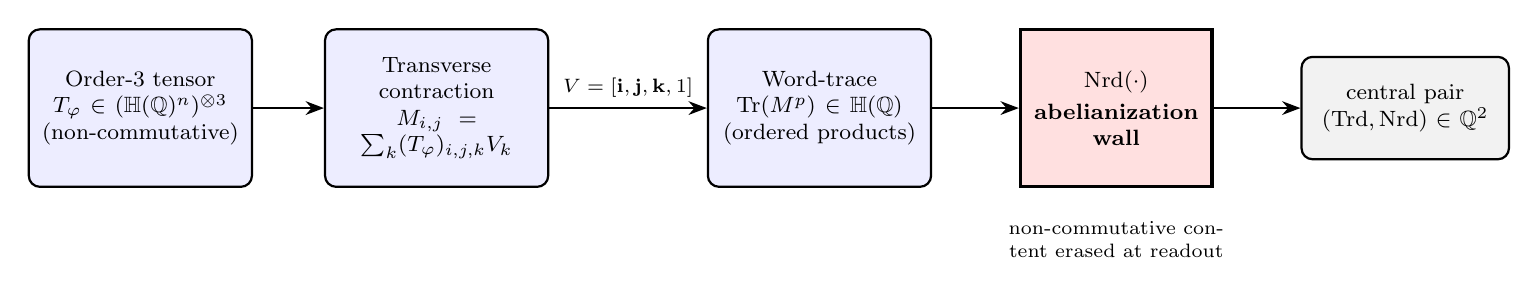
\begin{tikzpicture}[
  >=Stealth,
  blk/.style={rectangle,draw,thick,rounded corners,align=center,
              minimum height=20mm,text width=26mm,fill=blue!7,font=\footnotesize},
  wall/.style={rectangle,draw,very thick,align=center,
               minimum height=20mm,text width=22mm,fill=red!12,font=\footnotesize},
  res/.style={rectangle,draw,thick,rounded corners,align=center,
              minimum height=13mm,text width=24mm,fill=gray!10,font=\footnotesize},
  lbl/.style={font=\scriptsize}
]
\node[blk] (T) {Order-3 tensor\\ $\Tphi\in(\HH(\QQ)^n)^{\otimes3}$\\ (non-commutative)};
\node[blk,right=9mm of T] (M) {Transverse contraction\\ $M_{i,j}=\sum_k(\Tphi)_{i,j,k}V_k$};
\node[blk,right=20mm of M] (W) {Word-trace\\ $\Tr(M^p)\in\HH(\QQ)$\\ (ordered products)};
\node[wall,right=11mm of W] (N) {$\Nrd(\cdot)$\\[2pt] \textbf{abelianization wall}};
\node[res,right=11mm of N] (Q) {central pair\\ $(\Trd,\Nrd)\in\QQ^2$};

\draw[->,thick] (T) -- (M);
\draw[->,thick] (M) -- node[lbl,above]{$V=[\bi,\bj,\bk,1]$} (W);
\draw[->,thick] (W) -- (N);
\draw[->,thick] (N) -- (Q);

% hatch marks on the wall to suggest a barrier
\begin{scope}[on background layer]
  \foreach \yy in {-0.7,-0.4,...,0.8}{
    \draw[red!45,thick] ($(N.center)+(-0.9,\yy)$) -- ($(N.center)+(-0.55,\yy+0.35)$);
  }
\end{scope}

\node[lbl,align=center,below=3mm of N,text width=30mm]
  {non-commutative content erased at readout};
\end{tikzpicture}%
}
\caption{The extrinsic terminal abelianization
(Theorem~\ref{thm:terminal}). The order-3 tensor and the contracted matrix
retain genuine non-commutative structure, and the ordered word-trace
$\Tr(M^p)$ is a full quaternion; but the terminal reduced norm $\Nrd$ is the
abelianization map $\HH(\QQ)^{\times}\to\QQ_{>0}$, which projects the trace
onto the conjugation-invariant central pair $(\Trd,\Nrd)\in\QQ^2$. The
oriented (non-commutative) information survives in the object yet is erased
by the measurement---the ``wall''.}
\label{fig:pipeline}
\end{figure}

\subsection{Mathematical requirements for escape}

Theorem~\ref{thm:terminal} identifies precisely what must change. Any
extraction of the form $g\circ\Nrd$ is barred; escape requires a $\QQ$- or
$\bar\QQ$-valued functional of $M$ (or of $\Tphi$ directly) that does
\emph{not} factor through the conjugation quotient
$\HH(\QQ)//\HH(\QQ)^{\times}\cong\QQ^2$. Two structural directions are
consistent with this:

\begin{enumerate}
\item \emph{Non-abelian boundary evaluation.} Retain the full quaternion
$\Tr(M^p)=a+b\bi+c\bj+d\bk$ and study a functional that depends on the
oriented triple $(b,c,d)$, not merely on $b^2+c^2+d^2$---for instance a
\emph{tuple} of coordinated traces $\{\Tr(M^{p_1}),\dots,\Tr(M^{p_r})\}$
compared through their relative imaginary directions, which are \emph{not}
individually conjugation-invariant but whose relative configuration can be.
\item \emph{Non-local contraction.} Replace the local, linear marginal
\eqref{eq:contract} by a contraction that couples two hyperedges through a
shared variable, so that the invariant depends on the sign interference
between overlapping clauses---the smallest object able to see logical, as
opposed to connectivity, structure. Remark~\ref{rem:honest} shows that at
present the surviving signal is driven by vertex degree (connectivity), and
a formula and its polarity re-labellings share that connectivity while
differing in satisfiability; only an invariant sensitive to cross-clause
sign interference can distinguish them.
\end{enumerate}

\subsection{Status of the program}

We reiterate that no separation of $\mathrm{P}$ from $\mathrm{NP}$ is
claimed or approached. The contribution is a pair of exact structural
theorems delimiting \emph{why} an entire, natural family of local,
low-degree, quaternionic invariants cannot separate the $3$-SAT variety
from its complement, together with an exact, reproducible laboratory (QIL,
Section~\ref{sec:software}) that
functions as a falsification harness: it does not merely fail to find an
obstruction; it proves, over exact arithmetic, the structural reason a whole
class of candidates must fail. The boundary conditions established
here---avoid two-colourable bilinear formats (else intrinsic gauge
collapse), and avoid terminally-abelianized readouts (else extrinsic
abelianization)---delimit constraints that any successor invariant in this
vein must satisfy, in the spirit of GCT-style obstruction
searches~\cite{GCT1,GCT2}.

\newpage

%=======================================================================
\section{Research Software and Reproducibility}\label{sec:software}
%=======================================================================

All results in this paper are accompanied by the \emph{Quaternionic
Invariant Laboratory} (QIL), an open-source, exact-arithmetic research
framework. QIL is not an appendix to the paper but the official laboratory of
the research program: it is the environment in which every quaternionic
computation, tensor construction, invariant evaluation and reproducible
experiment reported here was carried out. The complete workspace---Rust
library, experiment drivers, manuscript sources, and documentation---is
publicly available at
\href{\QILRepositoryURL}{\nolinkurl{\QILRepositoryURL}}.

\subsection{What QIL is, and why it was built}

QIL is a Rust library and experiment suite that implements, exactly, the
mathematical objects of this manuscript. It was developed to make the
program's claims \emph{machine-checkable rather than merely asserted}: because
$3$-SAT satisfiability is combinatorial and finite, and because a spurious
low-complexity separating functional would be an artifact worth guarding
against, every invariant is computed over the exact rationals and every
published constant is re-derived by an automated check. The library is
organised so that each module corresponds to a concept of the paper: the
Hamiltonian division ring $\HH(\QQ)$; the two models (incidence matrix and
order-3 hypergraph tensor); the invariants (Dieudonn\'e determinant,
word-trace spectra, tensor invariants); the two collapse mechanisms
(intrinsic gauge collapse and extrinsic terminal abelianization); the exact
generators; and reproducible input/output.

\subsection{How QIL guarantees reproducibility}

Three design choices underwrite bit-for-bit reproducibility. First, there is
\emph{no floating-point arithmetic anywhere}: all coefficients are
arbitrary-precision integers and rationals, so a reduced norm such as
$\Nrd = 2^{16}$ or a tensor entry such as $660 + 660\bi + 660\bj$ is an exact
value, not an approximation. Second, all randomness is a deterministic
integer \texttt{SplitMix64} stream seeded by fixed constants, so a given
experiment reproduces identically on any platform. Third, ground-truth
satisfiability labels come from an exhaustive exact solver over all $2^n$
assignments, not a heuristic. The two data tables of
Section~\ref{sec:experiments} are emitted verbatim by
\[
  \texttt{cargo run -{}-example reproduce\_table\_1},\qquad
  \texttt{cargo run -{}-example reproduce\_table\_2},
\]
the contrast data behind the figures by
\texttt{cargo run -{}-example reproduce\_figures}, and the pinned constants
(e.g.\ the minimal-pair reduced norms $2^{16}$ and $2^{8}\cdot 13^{2}$) are
re-verified by \texttt{cargo run -{}-example exact\_validation}.

\subsection{Extending QIL}

QIL is designed as an extensible platform rather than a single-paper script.
New invariants are added by implementing a method on the relevant model in the
\texttt{invariants} module; new algebraic carriers (further non-commutative
algebras, higher-order tensors) slot into \texttt{algebra} and \texttt{models}
without disturbing existing code; and new experiments are added as
self-contained example drivers. The two collapse mechanisms of this paper are
implemented in the \texttt{collapse} module precisely so that a candidate
successor invariant can be tested against both barriers---avoidance of a
two-colourable bilinear format, and avoidance of a terminally-abelianized
readout---before it is trusted. QIL will be maintained as the reproducible
research platform for the future publications of this program.

%=======================================================================
\section{Conclusion and Roadmap}\label{sec:conclusion}
%=======================================================================

We have unified two phases of a single research program into one narrative
governed by a single question and answered it with two theorems. The
quaternionic incidence matrix collapses because its bipartite bilinearity
\emph{is} a diagonal gauge involution (Theorem~\ref{thm:collapse}), a defect
we proved intrinsic to the entire class of two-colourable order-$2$ formats
(Theorem~\ref{thm:intrinsic}) and hence unavoidable without raising the
carrier's arity to match the clause width (Corollary~\ref{cor:necessity}).
The resulting symmetric order-$3$ tensor is free of that gauge
(Proposition~\ref{prop:nogauge}) and does retain genuine non-commutative
structure once degree heterogeneity defeats the Fourier hypercube
annihilation (Theorem~\ref{thm:annih}, Proposition~\ref{prop:survive}), yet
its natural scalar invariants collapse a second time---not as a symmetry of
the object but as an abelianization of the readout
(Theorem~\ref{thm:terminal}), a phenomenon we illustrated on exact
size-matched data (Observation~\ref{obs:interleave}) and that illustrates,
in miniature, a collapse mechanism structurally analogous to the
algebrization barrier~\cite{AW}.

The roadmap follows from Theorem~\ref{thm:terminal}: any next step must both
(i) keep the object away from two-colourable bilinear formats and (ii) read
it out through a functional that does not factor through the reduced norm,
i.e.\ a non-abelian boundary evaluation or a non-local contraction sensitive
to cross-clause sign interference. Whether such an invariant of
$\Tphi$ resists both collapses and supplies an explicit obstruction is, in
our view, the sharply posed continuation of this line of inquiry; the two
negative theorems established here delimit exactly why the linear and the
locally-contracted stages were insufficient, and exactly what a successful
successor must not do.

\subsection*{Reproducibility}

\begin{sloppypar}
All assertions are exact statements over $\ZZ$ and $\QQ$ realised in the
Quaternionic Invariant Laboratory (QIL, Section~\ref{sec:software}) with
arbitrary-precision arithmetic and no floating point.
The principal constructions are \texttt{build\_from\_cnf}
(Definition~\ref{def:matrix}), \texttt{compute\_dieudonne\_determinant} and
\texttt{dieudonne\_reduced\_norm} (Construction~\ref{con:ddet}),
\texttt{build\_tensor\_from\_cnf} (Definition~\ref{def:assembly}),
\texttt{contract\_axis} (Definition~\ref{def:contract}),
\texttt{word\_trace} and \texttt{compute\_normalized\_invariant}
(Definition~\ref{def:invariants}), with the exact solver
\texttt{is\_satisfiable} and the deterministic generator
\texttt{random\_3cnf} supplying the labelled corpus of
Section~\ref{sec:experiments}.
\end{sloppypar}

\newpage
\bibliography{sn-bibliography}

\end{document}
